\documentclass{beamer}
\usepackage[english,russian]{babel}
\usepackage[utf8]{inputenc}
\usepackage{pagenumber}

\usepackage{hyperref}
% Стиль презентации
\usetheme[numbers, totalnumbers]{Dresden}
% цветовая схема
\usecolortheme{beaver}

\makeatletter
\defbeamertemplate*{footline}{Dresden}{
	\leavevmode%
	\hbox{%
	\begin{beamercolorbox}[wd=0.88\paperwidth,ht=2.25ex,dp=1ex,center]{title in head/foot}%
		\usebeamerfont{title in head/foot}\inserttitle
	\end{beamercolorbox}%
	\begin{beamercolorbox}[wd=.12\paperwidth,ht=2.25ex,dp=1ex,right]{date in head/foot}%
		\usebeamerfont{date in head/foot}\hspace*{2em}
		\insertframenumber{} / \inserttotalframenumber\hspace*{2ex}
	\end{beamercolorbox}}%
}
\makeatother

\begin{document}
\title{Пространственно-кинематическое моделирование однородной плоской подсистемы Галактики}  
\author{Д.В. Волков}
\institute{научный руководитель И.И. Никифоров \\ Санкт-Петербургский государственный университет }
\date{кафедра небесной механики, \\ \today} 
% Создание заглавной страницы
\frame{\titlepage} 

\begin{frame}{Предположения}
	\begin{itemize}
		\item Средняя линейная скорость $\Theta$ вращения подсистем Галактики -- функция от $R$: $\Theta = \Theta (R)$.
		\item Компоненты остаточного движения Солнца $u_{\odot}, v_{\odot}, w_{\odot}$ предполагаются заранее неизвестными и находятся вместе с другими параметрами модели.
                \item $K = 0$.
                \item Порядок разложения $n$ аппроксимирующих закон вращения полиномов считается заранее неизвестным и оптимизируется в ходе решения.
                \item Невязки (отклонения) наблюдаемых от модельных скоростей распределены по нормальному закону с нулевым математическим ожиданием. 
	\end{itemize}
\end{frame}

\begin{frame}{Кинематическая модель}
Для представления $\Theta(R)$ используем модельный полином в виде многочлена Тейлора:
	\begin{equation}
		\Theta_n(R) = \sum^n_{k = 0} \frac{\theta_k}{k!} \left( \Delta R \right)^k,
	\end{equation}
где
\begin{equation}
        \Delta R = R - R_0, ~\theta_k = \frac{d^k\Theta}{dR^k},
\end{equation}
\begin{equation}
	R = \sqrt{R_0^2 + r^2 \cos^2{b} - 2R_0 r \cos{l} \cos{b}}.
\end{equation}
\end{frame}

\begin{frame}{Лучевые скорости}
\begin{equation}
        V_{r, \mathrm{mod}} = (\omega - \omega_0) R_0 \sin{l} \cos{b} - V_{r, \odot},
\end{equation}
где $\omega$ и $\omega_0$ -- угловые скорости вращения подсистемы на $R$ и $R_0$, $l$ -- галактическая долгота, $b$ -- галактическая широта, $r$ -- гелиоцентрическое расстояние, $V_{r, \odot}$ -- проекция остаточной скорости движения Солнца.
	\begin{equation}
		V_{r, \mathrm{mod}} = \left[ -2A\Delta R + \sum^n_{k = 2} \frac{\theta_k}{k!} \left( \Delta R \right)^k \right] \frac{R_0}{R} \sin{l} \cos{b} + V_{r, \odot},
	\end{equation}
	\begin{equation}
		A = - \frac{1}{2} R_0 \omega^{'}(R_0) = - \frac{1}{2} (\theta_1 - \omega_0).
	\end{equation}
\end{frame}

\begin{frame}{Собственные движения}
Аналогично
\begin{equation}
        \mu_{l, \mathrm{mod}} = (\omega - \omega_0) \left( \frac{R_0\cos{l}}{r} - \cos{b} \right) - \omega_0 \cos{b} + \mu_{l, \odot},
\end{equation}
\begin{equation}
        \mu_{b, \mathrm{mod}} = - (\omega - \omega_0) \frac{R_0}{r} \sin{l} \sin{b} + \mu_{b, \odot}.
\end{equation}

\end{frame}


\begin{frame}{Собственные движения по широте}
Для собственных движений $\mu_b = \frac{db}{dt}$:
	\begin{equation}
		k\mu_{b, \mathrm{mod}} = k\mu_{b, \mathrm{rot}} + k\mu_{b, \odot},
	\end{equation}
	\begin{equation}
		k\mu_{b, \mathrm{mod}} = \left[ 2A\Delta R - \sum^n_{k = 2} \frac{\theta_k}{k!} \left( \Delta R \right)^k \right] \frac{R_0}{Rr} \sin{l} \sin{b},
	\end{equation}
	\begin{equation}
                k\mu_{b, \odot} = \frac{u_{\odot}\cos{l}\sin{b} + v_{\odot}\sin{l}\sin{b} - w_{\odot}\cos{b}}{r}.
	\end{equation}
        Здесь и далее полагаем $k=4.7406$.
\end{frame}

\begin{frame}{Собственные движения по долготе}
Для собственных движений $\mu_l = \frac{dl}{dt}\cos{b}$:
	\begin{equation}
		k\mu_{l, \mathrm{mod}} = k\mu_{l, \mathrm{rot}} + k\mu_{l, \odot},
	\end{equation}
	\begin{equation}
                k\mu_{l, \mathrm{mod}} = \left[ -2A\Delta R + \sum^n_{k = 2} \frac{\theta_k}{k!} \left( \Delta R \right)^k \right] \left( \frac{R_0\cos{l}}{r} - \cos{b} \right) R^{-1} - \omega_0 \cos{b},
	\end{equation}
	\begin{equation}
                k\mu_{b, \odot} = \frac{u_{\odot}\sin{l}- v_{\odot}\cos{l}}{r}.
	\end{equation}
\end{frame}

\begin{frame}{Метод}
	Решаются системы уравнений
	\begin{equation}
                V_r = V_{r, \mathrm{mod}} (R_0, A, \theta_2, \:\ldots,\: \theta_n, u_{\odot}, v_{\odot}, w_{\odot}^{*}),
	\end{equation}
	\begin{equation}
                k\mu_l = k\mu_{l, \mathrm{mod}} (R_0^{*}, A, \omega_0, \theta_2, \:\ldots,\: \theta_n, u_{\odot}, v_{\odot}),
	\end{equation}
	\begin{equation}
                k\mu_b = k\mu_{b, \mathrm{mod}} (R_0^{*}, A, \theta_2, \:\ldots,\: \theta_n, u_{\odot}, v_{\odot}, w_{\odot}).
	\end{equation}
        Параметры со звездочкой могут фиксироваться. Каждая из систем решается обычным МНК с единичными весами.
\end{frame}

\begin{frame}{Метод}
Найденные общие решения дают оценки дисперсий:
	\begin{equation}
                \sigma^2_{V_r} = \frac{1}{N_{\mathrm{free}}} \sum^N_{i = 1} \left( V_r - V_{r, \mathrm{mod}} \right)^2_i,
	\end{equation}
	\begin{equation}
                \sigma^2_{\mu_l} = \frac{1}{N_{\mathrm{free}}} \sum^N_{i = 1} \left( k\mu_l - k\mu_{l, \mathrm{mod}} \right)^2_i,
	\end{equation}
	\begin{equation}
                \sigma^2_{\mu_b} = \frac{1}{N_{\mathrm{free}}} \sum^N_{i = 1} \left( k\mu_b - k\mu_{b, \mathrm{mod}} \right)^2_i,
	\end{equation}
        где число степеней свободы $N_{\mathrm{free}} = N - n_{\mathrm{par}}$, $n_{\mathrm{par}}$ -- количество параметров модели.
\end{frame}

\begin{frame}{Метод}
\textit{Природная дисперсия} $\sigma_0$ объектов подсистемы -- дисперсия скоростей, объективно существующая вне зависимости от ошибок наблюдений. Минимизируется целевая функция
\begin{equation} \label{chi_sq_func}
        \chi^2 = \sum^N_{i = 1} \left[ \frac{\left( V_r - V_{r, \mathrm{mod}} \right)^2_i}{\sigma_0^2 + \sigma^2_{V_{r_i}}} + \frac{\left(k \mu_l - k\mu_{l, \mathrm{mod}} \right)^2_i}{\frac{\sigma_0^2}{r_i^2} + k^2\sigma^2_{\mu_{l_i}}} + \frac{\left(k \mu_b - k\mu_{b, \mathrm{mod}} \right)^2_i}{\frac{\sigma_0^2}{r_i^2} + k^2\sigma^2_{\mu_{b_i}}} \right].
\end{equation}

\par Здесь $\sigma_{V_{r_i}}$, $\sigma_{\mu_{l_i}}$, $\sigma_{\mu_{b_i}}$ -- ошибки измерения лучевых скоростей и собственных движений.

\begin{equation}
        \chi^2(\sigma_0) |_{\sigma_{0, \mathrm{opt}}} = N_{\mathrm{free}} = 3 N - n_{\mathrm{par}}.
\end{equation}
\end{frame}


\begin{frame}{Выбор оптимального порядка полинoма}
	Критерии:
	\begin{itemize}
		\item Значимость старших коэффициентов.
		\item Зависимость дисперсии от порядка.
		\item Наличие краевых эффектов у кривой вращения для данного порядка.
                \item Гладкость профиля (зависимости $\chi^2(R_0)$) целевой функции для параметра $R_0$ .
                \item Связность линий равной плотности маргинальных распределений параметров.
	\end{itemize}
\end{frame}

\begin{frame}{Исключение по невязкам}
	\begin{itemize}
		\item Для данной мощности выборки вычисляется значение $\kappa$
			\begin{equation}
				\big(1 - \psi(\kappa)\big) N = 1,
			\end{equation}
			где $\psi(\kappa)$ -- интеграл
			\begin{equation}
				\psi(\kappa) = \sqrt{\frac{2}{\pi}} \int^{\kappa}_{0} e^{-\frac{1}{2}t^2} dt.
			\end{equation}
		\item Исключаются объекты с невязками
			\begin{equation}
				\frac{| \varepsilon_i |}{\sigma_i} > \kappa
			\end{equation}
	\end{itemize}
Далее находится количество уравнений $L$, удовлетворяющих условию. Если $L > 1$, то из дальнейшего рассмотрения исключается $L - 1$ уравнений с наибольшими по модулю невязками. 
\end{frame}



\begin{frame}{Наблюдательные данные}
        Красное сгущение -- скопление красных гигантов на диаграмме Герцшпрунга-Рассела при температуре ок. 5000 K и абсолютной зв. величине +0.5. Пачыньски и Станек выдвинули звезды красного сгущения как новый индикатор расстояний.
	\begin{center}
	\begin{figure}[h]
\begin{minipage}[h]{0.8\linewidth}
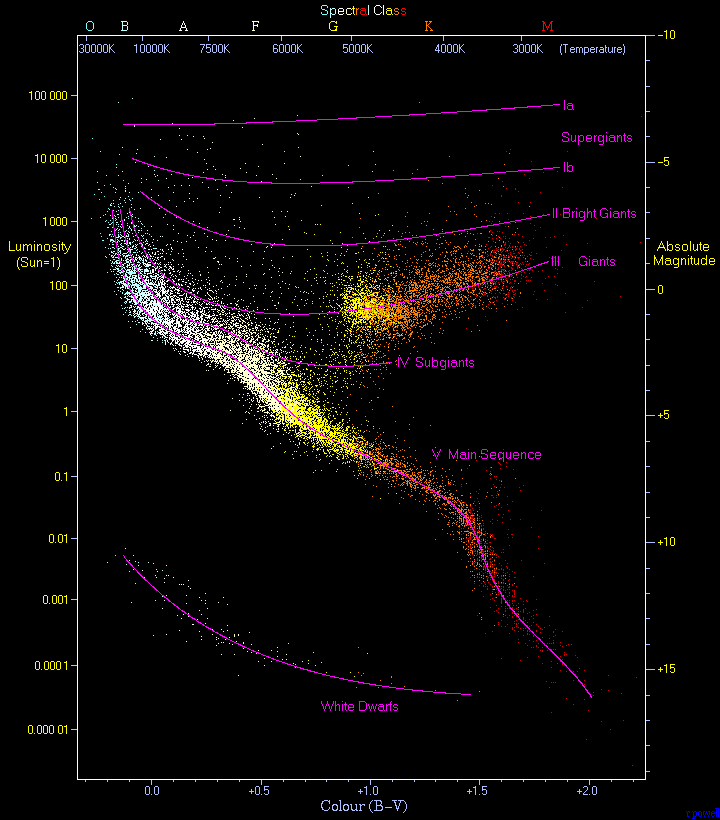
\includegraphics[width=1\linewidth]{../imgs/HRDiagram.png}
\end{minipage}
\end{figure}
	\end{center}

%        \begin{itemize}
%		\item 29502 объекта.
%		\item Очень точные данные о лучевых скоростях.	
%                \item Имеются данные для собственных движений для большинства объектов (UCAC-4, HSOY)
%		\item Точность измерения гелиоцентрических расстояний.
%		\item Каталог обновляется.
%	\end{itemize}
\end{frame}


\begin{frame}{APOGEE-RC}
        Apache Point Observatory Galactic Evolution Experiment (APOGEE) представляет собой спектроскопическую съемку в ближней инфракрасной области с высоким разрешением, охватывающую все основные компоненты Галактики, в том числе непроницаемые из-за пыли области внутреннего диска Млечного Пути и балджа. Каталог RC (Red Clump)  -- это выборка из более чем 29 тыс. звезд, полученная по результатам Bovy, 2014. Метод определения расстояний имеет точность от $5$ до $10\%$ (была использована калибровка ЗКС $M_{K_s} = -1.613 \pm 0.015 $ из работы Laney(2012), которая на 0.07 mag ярче, чем у Groenewegen, 2008). Каталог содержит гелиоцентрические расстояния и лучевые скорости, и собственные движения из каталогов UCAC-4 и HSOY (Hot Stuff for One Year). 
\end{frame}



\begin{frame}{APOGEE-RC}

\begin{figure}[h!]
\begin{minipage}[h]{0.49\linewidth}
        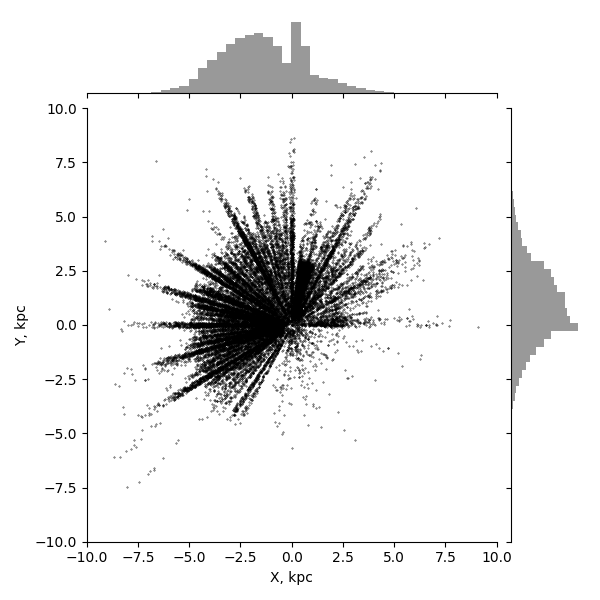
\includegraphics[width=0.95\textwidth]{../imgs/XYobj.png}
\end{minipage}
\hfill
\begin{minipage}[h]{0.49\linewidth}
        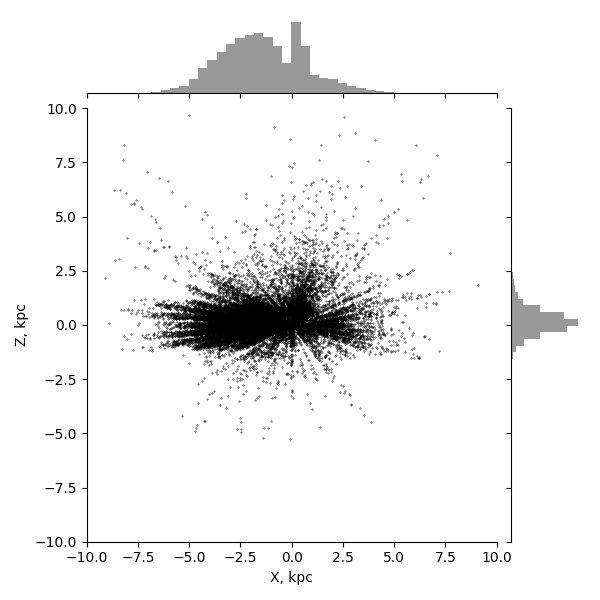
\includegraphics[width=0.95\textwidth]{../imgs/XZobj.png}
\end{minipage}
\caption{Распределение объектов APOGEE-RC в гeлиоцентрических декартовых координатах. Ось $X$ ориентирована на Центр Галактики. }
\end{figure}


\end{frame}



\begin{frame}{APOGEE-RC}

Лучевые скорости измерены с высокой точностью.

\begin{figure}[h!]
\begin{minipage}[h]{0.49\linewidth}
        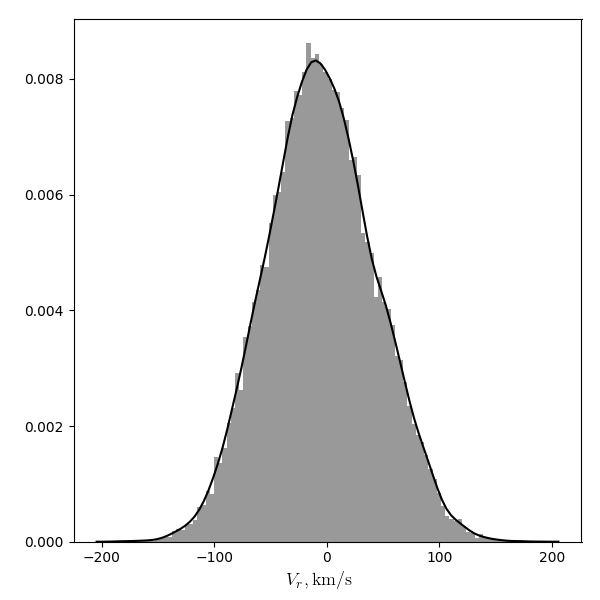
\includegraphics[width=0.95\textwidth]{../imgs/vr_distr.png}
\end{minipage}
\hfill
\begin{minipage}[h]{0.49\linewidth}
        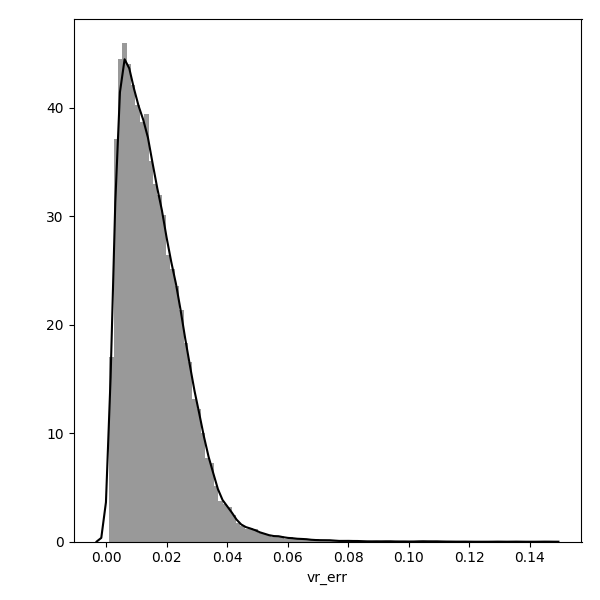
\includegraphics[width=0.95\textwidth]{../imgs/vr_err_distr.png}
\end{minipage}
\caption{Распределение лучевых скоростей и их измертельных ошибок.}
\end{figure}
\end{frame}



\begin{frame}{APOGEE-RC}
	\begin{center}
	\begin{figure}[h]
\begin{minipage}[h]{0.8\linewidth}
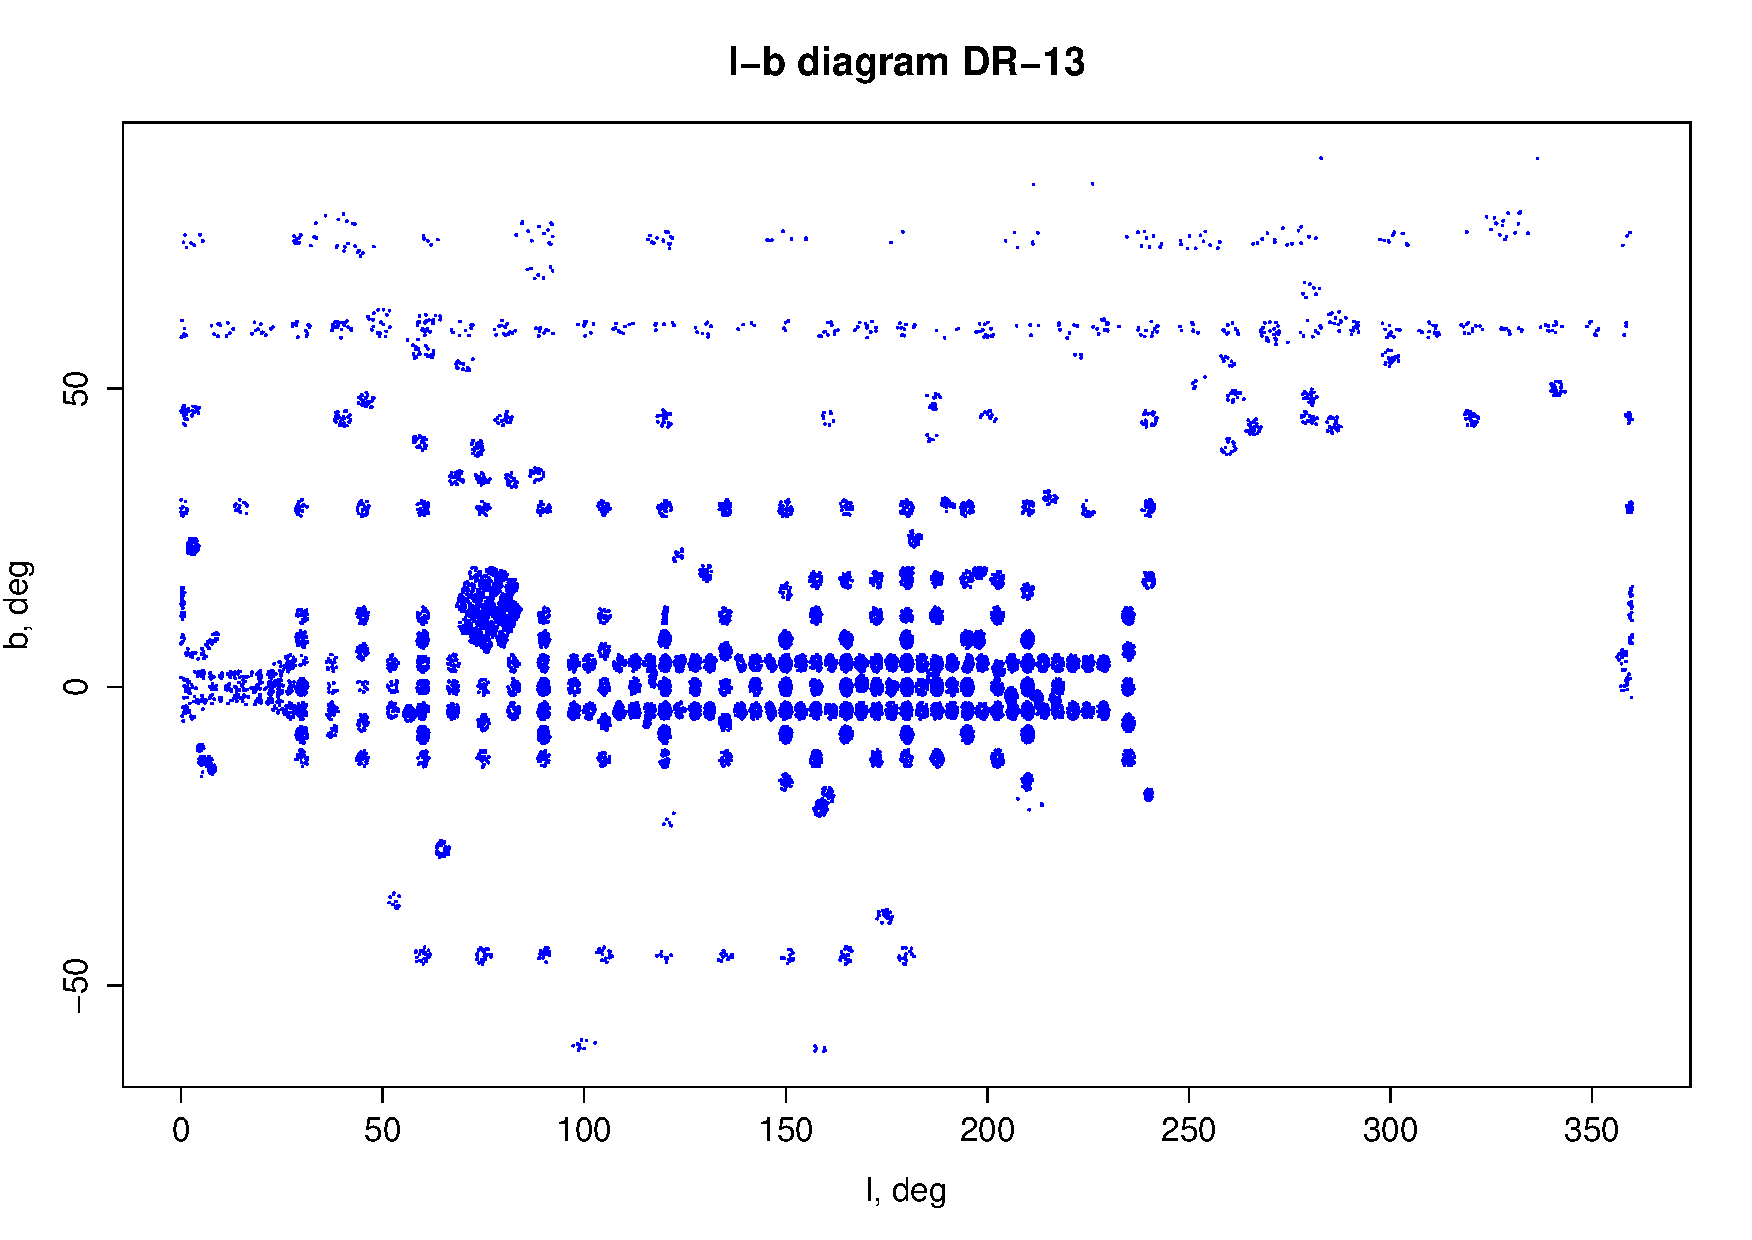
\includegraphics[width=1\linewidth]{pdf/lb_dr13.pdf}
\end{minipage}
\end{figure}
	\end{center}
\end{frame}
\begin{frame}{Зависимость дисперсии от порядка}
\begin{figure}[h]
\begin{minipage}[h]{0.8\linewidth}
	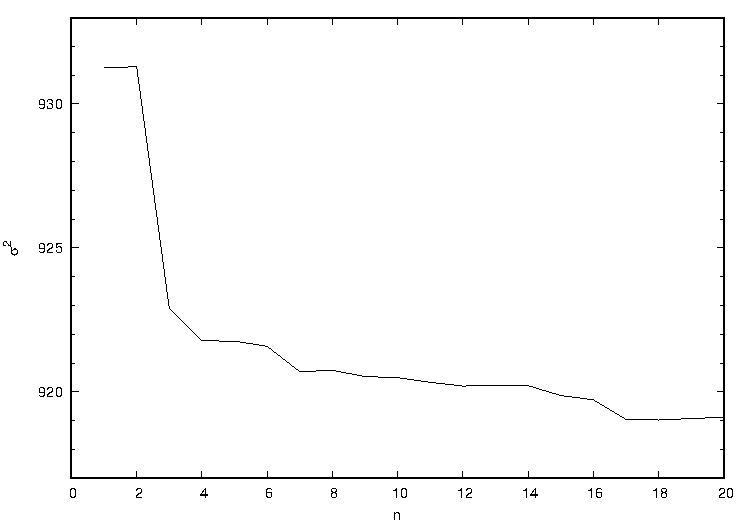
\includegraphics[width=1\linewidth]{pdf/sigmas.pdf}
\end{minipage}
\end{figure}
\end{frame}
\begin{frame}{Результаты}
	\begin{table}[ht]
	\centering
\begin{tabular}{r|r}
  \hline
  $n$& $3$\\
  \hline
  $R_0$, \texttt{кпк} & $7.40^{+0.18^{\vphantom{T^T}}}_{-0.11} $ \\
  \hline
  $\chi^2_*$& $81438$ \\
  \hline
  $N_{free}$& $81905$ \\
  \hline
  $N$& $28450$ \\
  \hline
  $u_0$, \texttt{км/с}  & $12.68 \pm 0.46 $ \\
  $v_0$, \texttt{км/с} & $25.78 \pm 0.61$ \\
  $w_0$, \texttt{км/с}  & $6.71 \pm 0.62$ \\
  \hline
  $A$, \texttt{км/с/кпк} & $ 13.34 \pm 0.30 $ \\
  \hline
  $\omega_{0}$, \texttt{км/с/кпк} & $ 28.08 \pm 0.54 $ \\
  \hline
\end{tabular}
\end{table}
\end{frame}

\begin{frame}{Кривая вращения для $n = 3$}
\begin{figure}[h]
\begin{minipage}[h]{0.8\linewidth}
	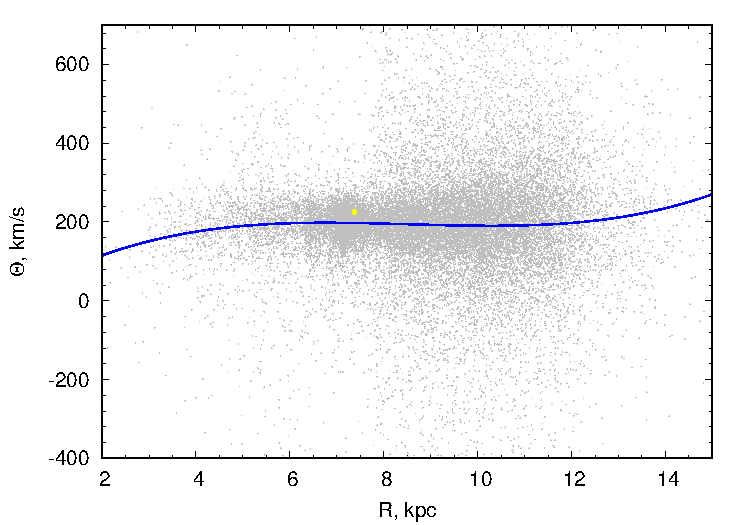
\includegraphics[width=1\linewidth]{pdf/rotc.pdf}
\end{minipage}
\end{figure}
\end{frame}

\begin{frame}{Заключение}
	\begin{itemize}
		\item Реализация алгоритма решения систем уравнений кинематической модели плоской подсистемы с исключением по избыточным невязкам в нескольких вариантах методом МНК.
		\item Исследование подсистемы звезд красного сгущения по данными каталога APOGEE-RC DR-14.
		\item Определение расстояния до центра Галактики, основных параметров движения Солнца в Галактике и параметров кинематической модели.
	\end{itemize}
\end{frame}


\begin{frame}{Ссылки}
 \begin{thebibliography}{10}
\beamertemplatebookbibitems
\bibitem{1} {\sc APOGEE-RC} {\em https://data.sdss.org/sas/dr13/apogee/vac/apogee-rc/cat/}
\bibitem{2} {\sc Bovy and etc.} {\em http://adsabs.harvard.edu/abs/2014arXiv1405.1032B}
\bibitem{3} {\sc Loktin A. V., Marsakov V. A. 2010} {Lectures on Stellar Astronomy, Rostov-na-Donu, pp. 282 (in Russian)}
\bibitem{3} {\sc Gromov A.O., Nikiforov I.I. 2016} {STÄCKEL-TYPE DYNAMIC MODEL OF THE GALAXY BASED
ON MASER KINEMATIC DATA}

\end{thebibliography}
\end{frame}

\end{document}
